\documentclass[a4paper,14pt]{extarticle}
\usepackage{../../tex-shared/report-layout}

\renewcommand{\mylabnumber}{1}
\renewcommand{\mylabtitle}{Исследование применения аппарата
бинарных отношений для решения задачи выбора альтернатив}
\renewcommand{\mysubject}{Теория принятия решений}
\renewcommand{\mylecturer}{Кротов К. В.}

\begin{document}
\begin{titlepage}
    
    \thispagestyle{empty}
    
    \begin{center}
        
        Министерство науки и высшего образования Российской Федерации \\
        Севастопольский государственный университет \\
        Кафедра ИС
        
        \vfill

        Отчет \\
        по лабораторной работе №\mylabnumber \\
        \enquote{\mylabtitle} \\
        по дисциплине \\
        \enquote{\MakeTextUppercase{\mysubject}}

        \vspace{2cm}

        \begin{tabular}{ | c | c | }
            \hline
            \hspace{7cm} & \hspace{7cm} \\
            \hspace{7cm} & \hspace{7cm} \\
            \hline
        \end{tabular}

    \end{center}

    \vspace{1cm}

    \noindent\hspace{7.5cm} Выполнил студент группы ИС/б-17-2-о \\
    \null\hspace{7.5cm} Горбенко К. Н. \\
    \null\hspace{7.5cm} Проверил \\
    \null\hspace{7.5cm} \mylecturer

    \vfill

    \begin{center}
        Севастополь \\
        2020
    \end{center}

\end{titlepage}

\section{Цель работы}
Исследовать применение аппарата бинарных отношений при принятии решений по
выбору альтернатив.

\section{Задание на работу}

\begin{enumerate}
    \item Для \textbf{Варианта 1} задания на работу, связанного с формированием
          подмножества максимальных элементов MaxR множества Х, необходимо по
          заданному варианту графа отношений предпочтения между решениями
          сформировать матрицу А отношения R (где R – отношение
          $\succ$). При этом убедиться, что первый элемент множества Х
          является строго независящим от других решений.

    \item Выполнить формирование множества MaxR вручную для заданного вида графа
          и соответствующего ему вида матрицы А.

    \item Выполнить формирование программного кода соответствующей процедуры
          определения множества MaxR, при этом возможно руководствоваться
          ориентировочным видом процедуры определения этого множества,
          предложенным в теоретическом введении данной лабораторной работы.

    \item Выполнить вывод результатов работы процедуры и сравнить полученные в
          процедуре результаты с результатами, сформированными аналитически.

    \item Изменить исходные данные программы, используя графы отношений из
          примера 5 (Рис 7). Проверить получаемые с использованием процедуры
          результаты с аналитическим результатами, формируемыми для этих графов.
\end{enumerate}

\section{Ход работы}
\subsection{Матрица отношений}
Сформируем матрицу отношения $\succ$ для графа отношений, соответствующего
варианту № 1, изображенного на рисунке \ref{fig:variant-graph}.

\begin{figure}[H]
    \centering
    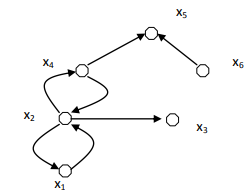
\includegraphics[width=.5\linewidth]{variant-graph}
    \caption{Граф отношений варианта № 1}
    \label{fig:variant-graph}
\end{figure}

Матрица отношения выглядит следующим образом:

$$\begin{pmatrix}
    0, 1, 0, 0, 0, 0 \\
    1, 0, 1, 1, 0, 0 \\
    0, 0, 0, 0, 0, 0 \\
    0, 1, 0, 0, 1, 0 \\
    0, 0, 0, 0, 0, 0 \\
    0, 0, 0, 0, 1, 0
\end{pmatrix}$$

\subsection{Ручное формирование множества $Max_R X$}
Рассмотрим каждую вершину графа, изображенного на рисунке
\ref{fig:variant-graph} на предмет включения во множество $Max_R X$.

\begin{enumerate}
    \item Решение x1 не является доминируемым, оно эквивалентно решениям x2 и
          x4, при этом ни одно решение не доминирует над ними. Из этого следует,
          что решения x1, x2 и x4 должны быть включены во множество $Max_R X$.

    \item Решение x3 доминируемо решением x2, в множество $Max_R X$ не включаем.
    
    \item Решение x5 доминируемо решениями x4 и x6, в множество $Max_R X$ не
          включаем.

    \item Решение x6 никаким решением не доминируемо и ни с каким решением не
    эквивалентно, включим его в множество $Max_R X$.
\end{enumerate}

Итоговое множество $Max_R X$ состоит из следующих элементов: x1, x2, x4 и x6.

\subsection{Реализация процедуры формирования множества $Max_R X$}
Реализованная процедура формирования множества $Max_R X$ приведена на следующем
листинге (полный программный код приведен в приложении):

\begin{lstlisting}
let private getMaxR (matrix: int list list): int list =
    let size = matrix |> List.length
    let maxR = [| for i in [0..size-1] do 1 |]

    for i in [0..size - 1] do
        for j in [0..size - 1] do
            if matrix.[i].[j] = 1 && matrix.[j].[i] = 0 then
                maxR.[j] <- 0
            if matrix.[j].[i] = 1 && maxR.[j] = 0 then
                maxR.[j] <- 0

    for i in [0..size - 1] do
        for j in [0..size - 1] do
            if matrix.[i].[j] = 1 && matrix.[j].[i] = 1 && maxR.[j] = 0 then
                maxR.[i] <- 0;

    maxR |> List.ofArray
\end{lstlisting}

Результат работы программы приведен на рисунке \ref{fig:variant-program-result}.
Множество $Max_R X$, сформированное с помощью программы совпадает со
сформированным ранее вручную.

\begin{figure}[H]
    \centering
    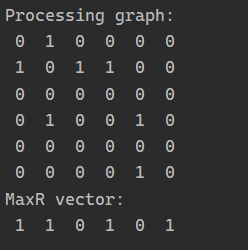
\includegraphics[width=.5\linewidth]{variant-program-result}
    \caption{Результат работы программы формирования множества максимальных решений}
    \label{fig:variant-program-result}
\end{figure}

\subsection{Проверка работы программы на графах рисунка 7}
Включим во входные данные программы матрицы отношений графов с рисунка 7:

\begin{lstlisting}
let picture7aRelationGraph = [
    [0; 0; 0; 1; 0]
    [0; 0; 1; 0; 0]
    [0; 0; 0; 1; 1]
    [0; 0; 1; 0; 0]
    [0; 0; 1; 0; 0]
]

let picture7bRelationGraph = [
    [0; 1; 0; 1; 0]
    [1; 0; 1; 0; 0]
    [0; 0; 0; 1; 1]
    [0; 0; 1; 0; 0]
    [0; 0; 0; 0; 0]
]
\end{lstlisting}

Результат работы программы для таких входных данных изображен на рисунке
\ref{fig:pic7-program-result}

\begin{figure}[H]
    \centering
    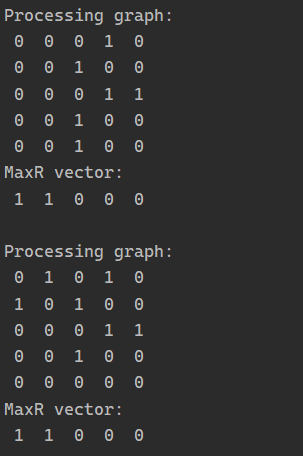
\includegraphics[width=.5\linewidth]{pic7-program-result}
    \caption{Результат работы программы формирования множества максимальных решений для графов с рисунка 7}
    \label{fig:pic7-program-result}
\end{figure}

Все результаты совпадают с аналитическими.

\section*{Выводы}

В ходе лабораторной работы была рассмотрена задача выбора оптимальных решений из
альтернатив с помощью аппарата бинарных отношений. В частности, была рассмотрена
ситуация, когда для списка альтернатив не может быть сформировано множество
предпочитаемых решений.

Для решения задачи было сформировано множество $Max_R X$ максимальных решений по
следующим правилам:

\begin{enumerate}
    \item решение исключается из $Max_R X$ если оно доминируемо другим решением;
    \item решение исключается из $Max_R X$ если оно эквивалентно другому решению, которое не включено в $Max_R X$;
    \item если решение ником не доминируемо, то оно включается в $Max_R X$.
\end{enumerate}

В результате максимальные множества, полученные аналитически и программно, совпали.

\newpage

\section*{Приложение}
Программный код приложения:

Файл Program.fs:

\begin{lstlisting}
module BinaryRelations.Program

open System

let private printMatrix (matrix: int list list): unit =
    let size = matrix |> List.length
    for i in [0..size - 1] do
        for j in [0..size - 1] do
            matrix.[i].[j] |> printf " %d " |> ignore
        printfn "" |> ignore

let private printVector (vector: int list): unit =
    vector |> List.iter (fun x -> x |> printf " %d " |> ignore)

let private getMaxR (matrix: int list list): int list =
    let size = matrix |> List.length
    let maxR = [| for i in [0..size-1] do 1 |]

    for i in [0..size - 1] do
        for j in [0..size - 1] do
            if matrix.[i].[j] = 1 && matrix.[j].[i] = 0 then
                maxR.[j] <- 0
            if matrix.[j].[i] = 1 && maxR.[j] = 0 then
                maxR.[j] <- 0

    for i in [0..size - 1] do
        for j in [0..size - 1] do
            if matrix.[i].[j] = 1 && matrix.[j].[i] = 1 && maxR.[j] = 0 then
                maxR.[i] <- 0;

    maxR |> List.ofArray

[<EntryPoint>]
let main (_: string array): int =
    let matrices = [
        Data.relationGraphByVariant
        Data.picture5RelationGraph
        Data.picture7aRelationGraph
        Data.picture7bRelationGraph
        Data.relationGraphWithNoDominatingAlternative
    ]

    matrices
    |> List.map (fun x -> x, getMaxR x)
    |> List.iter (fun x ->
            let matrix, maxR = x

            printfn "%sProcessing graph:" (String.replicate 2 Environment.NewLine) |> ignore
            matrix |> printMatrix
            printfn "MaxR vector:" |> ignore
            matrix |> getMaxR |> printVector
        )

    0
\end{lstlisting}

Файл Data.fs:

\begin{lstlisting}
module BinaryRelations.Data

let relationGraphByVariant = [
    [0; 1; 0; 0; 0; 0]
    [1; 0; 1; 1; 0; 0]
    [0; 0; 0; 0; 0; 0]
    [0; 1; 0; 0; 1; 0]
    [0; 0; 0; 0; 0; 0]
    [0; 0; 0; 0; 1; 0]
]

let picture5RelationGraph = [
    [0; 0; 1; 0; 0]
    [0; 0; 1; 0; 0]
    [0; 1; 0; 1; 1]
    [0; 0; 1; 0; 0]
    [0; 0; 0; 0; 0]
]

let picture7aRelationGraph = [
    [0; 0; 0; 1; 0]
    [0; 0; 1; 0; 0]
    [0; 0; 0; 1; 1]
    [0; 0; 1; 0; 0]
    [0; 0; 1; 0; 0]
]

let picture7bRelationGraph = [
    [0; 1; 0; 1; 0]
    [1; 0; 1; 0; 0]
    [0; 0; 0; 1; 1]
    [0; 0; 1; 0; 0]
    [0; 0; 0; 0; 0]
]

let relationGraphWithNoDominatingAlternative = [
    [0; 1; 0; 0; 0; 0; 0]
    [1; 0; 1; 0; 0; 0; 0]
    [0; 0; 0; 1; 0; 0; 0]
    [0; 0; 1; 0; 1; 1; 0]
    [0; 0; 0; 0; 0; 0; 0]
    [1; 0; 0; 1; 0; 0; 1]
    [0; 0; 0; 0; 0; 0; 0]
]
\end{lstlisting}

\end{document}